\chapter{Implementation and Testing}
Following the formal definition of the Lispish language and briefly describing the operations of the compiler, we shall dive into the construction of it. Along the way, I will explain the concepts behind most of the mechanics of the compiler. 

In the following sections, we will also test the implementation by means of examples of an actual compilation. 
At the end, we will look into automating the tests by means of using a Clojure testing API.  

\section{Building the compiler}
This section will describe the operations of the compiler and the fundamental concepts behind how the compiler translates the input Lispish code to JavaScript. 

Lispish translator is implemented as a single pass compiler.
This design decision comes from the fact that the compiler has been implemeneted in Clojure, which is a strictly functional language and in order to sustain the immutability property throughout the compiler and not violate common idioms, the compiler avoids using state at all costs. It was therefore difficult to perform multi-pass compilation over the same code, as it is done in other commercial compilers. 
As a consequence of this, the entire implementation is built around recursively invoking a set a functions, which at the end fold to yield a JavaScript string as a result. 



\subsection{Recursive Expansion}
The main idea behind the Lispish compiler's implementation is recursive expansion.
The compiler breaks down each s-expression that it comes across into its primitives until there is no more work to be done. It then builds up the result in layers as the recursion folds upwards. 

Figure ~\ref{fig:recursive_expansion_flowchart} illustrates the flow chart of the compiler. It covers most of the operations of the compiler, except for the details on how multi-arity s-expressions are handled.  

\begin{figure}[!htbp]
	\centering
	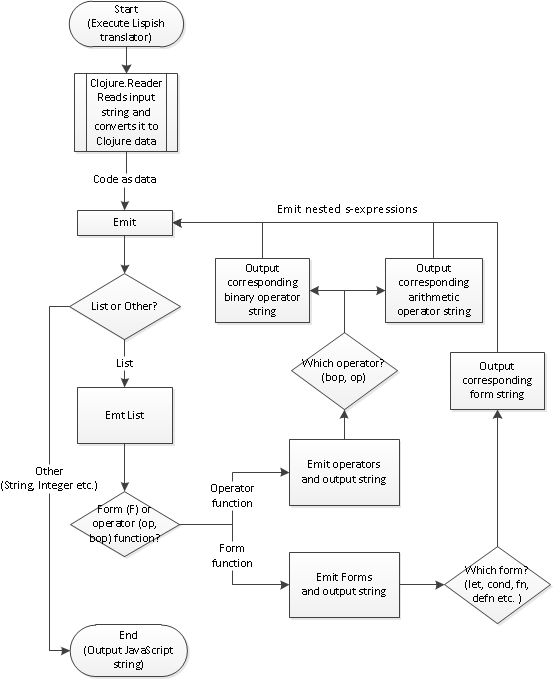
\includegraphics{Graphics/compilation_flow_chart.png}
	\caption[yadayada]
   {Flow chart of \textit{Lispish to JavaScript} compilation.}
  \label{fig:recursive_expansion_flowchart}
\end{figure}

\subsection{Forms with multiple arity}

In order to solve the multiple arity problem, where for instance a \texttt{(cond )} form can take multiple condition/true-form expression tuples and each one of them has to be compiler to a JavaScript string, map and reduce constructs have been used. 

\subsubsection{Map}
The idea behind the map operation is to apply a function that takes one argument, to all of the elements in a collection and return a new collection with results of each application of the aforementioned function. 
A simple example of Map is 

\begin{verbatim}
(map (fn [x] (+ x 1)) 
	 [0 1 2 3 4 5])
\end{verbatim}
that yields 
\begin{verbatim}
[1 2 3 4 5 6]
\end{verbatim}
as a result

\subsection{Reduce}
Reduce is a function that takes a function, an optional value (or an s-expression) and a collection as an argument. It reduces or in other words folds a given collection (and an optional value) through the application of a function to a collection, to a single result. 
\begin{verbatim}
(reduce 
   str
   1
	 [1 2 3])
\end{verbatim}
that yields 
\begin{verbatim}
"1123"
\end{verbatim}
as a result. The collection of numbers has been reduced to a string, as each number was converted to a string and then a string of the collection has been produced.
If we would to map a \texttt{str} function over the collection of \texttt{[1 2 3]}, it would result in a new collection containing all of the elements of the old collection converted to a string, namely the list \texttt{("1" "2" "3")}.

To now put the map reduce constructs into perspective with Lispish, figure ~\ref{fig:emit-cond-code} illustrates how a multiple arity cond (allowing practically unbound list of tests) is implemented.


\begin{figure}[ht]
\begin{verbatim}
(defn emit-cond [head [name & rest]]
  (let [rev (reverse (partition 2 rest))]
    (reduce
    	(fn [a b] (str "(" (emit (first b)) "?" (emit (second b)) ":" a ")"))
        (str (emit (second (first rev))))
        (drop 1 rev))))
\end{verbatim}
\caption{emit-cond source code}
\label{fig:emit-cond-code}
\end{figure}


Given an arbitrary number of \texttt{(test) result} tuples for the input 
\texttt{(cond )}, the \texttt{(emit-cond)} form first partitions the input into test and expression tuples, then reverses the tuples, so that the originally last one appears at the front, allowing us to perform a right reduce (right fold) and then binds it to a local \texttt{rev} variable. 
For example, if \texttt{(emit-cond )} is invoked with the following arguments:

$$ \texttt{(< 5 2) false (> 3 2) true :else false} $$

the content of the locally scoped \texttt{rev} will be 

$$ \texttt{((:else false) ((> 3 2) true) ((< 5 2) false))} $$

The reduce function then applies the anonymous function to the first value, which is the result of \texttt{(str (emit (second (first rev))))}, which in this example happens to be the \texttt{false} symbol, as it is grabbed from the first tuple \texttt{(:else false)} as the second element. Reduce is then applied to the second, third etc. element of the collection, in this case the \texttt{((> 3 2) true) ((< 5 2) false)}, whilst the overall result is accumulated in \texttt{a}.

\begin{figure}[ht]
\centering
\begin{tabular}{ r | l || l }
1. & \texttt{a: false} & \texttt{b: ((> 3 2) true)} \\
2. & \texttt{a: ((3>2)?true:false)} & \texttt{b: ((< 5 2) false)} \\
3. & \texttt{a: ((5<2)?false:((3>2)?true:false))} & b:
\end{tabular}
\caption{Reduction of a cond with multiple arguments}
\label{fig:emit-cond-expansion}
\end{figure}


Figure ~\ref{fig:emit-cond-expansion} illustrates a table of how each reduction step is performed in terms of the two arguments of the function passed to reduce. Variable \texttt{a} accumulates the overall result, whilst \texttt{b} is the current element of the \texttt{(cond )} that is being converted to JavaScript ternary expression.

\section{Testing}
The section above described the operations that are part of the compilation, but they did not provide any examples of an actual compilation. 
In this section we will take a look at some examples of how our Lispsh to JavaScript compiler works. 
To illustrate the compilation, I will demonstrate the output of the recursive expansion that the compiler performs on the given Lispish program string. 
Each line of the compilation trace will correspond to a level in the recursion. The recursion folding will be done implicitly, therefore it does not appear in the compilation traces. 

Let's begin our tests by a simple arithmetic expression:
\begin{verbatim}
lispish.core> (lisp-to-js "(+ 2 2)")
Emit Lispish:  (+ 2 2)
Emit-list head:  + , tail:  (2 2)
Emit-op, head:  + , tail:  (2 2)
Emit Lispish:  2
Emit Lispish:  2
"(2+2)"
\end{verbatim}
As we can see, our recursion begins with passing the Lispish source code to a lisp-to-js macro, which then begins the recursion by invoking the initial emit step.
At first, our s-expression is of the form (+ 2 2), which is a list. This means that the compiler has to expand the list and emit each individual expression within it. It begins by evaluating the head of the list, which happens to be an "op" operator, in this case the "+" sign. 
It therefore passes the head of the previous s-expression (the "+" sign), as well as the remaining part of the expression (2 2) to emit-op. 
Emit-op outputs the corresponding JavaScript by first mapping the top-level recursion emit function to each element inside of the tail list (2 2) which reaches the bottom of the recursion in one step each and then reduces the result of this to a string concatenated with the operator in the middle.
The same procedure is repeated for all of the "op", as well as "bop" expressions.

In the next sub section, we will have a look at a more complex example of generating a named function that is implemnted largely with Abstract Structural Binding.

\subsection{Abstract Structural Binding}
Abstract Structural Binding in simple words means de-structuring. It allows for de-structuring any data structure to a corresponding argument in function parameters or a let form, creating locally scoped bindings.
For example, if we define a let as follows:
\begin{verbatim}
(let [[x1 x2] [1 2]])
\end{verbatim}
"x1" will yield 1 and "x2" will yield 2.
The same principle is true for a function.
If our function accepts one parameter which is a collection:

\begin{verbatim}
(defn test [[x1 x2]] (println x1 x2))
(test [1])
\end{verbatim}
and it binds the first two elements of the collection to x1 x2, in the above case, x1 will yield 1 and x2 null.

Lispish uses de-structuring for generating all of its forms ($F$):
\begin{verbatim}
lispish.core> (lisp-to-js (defn square [x] (* x x)))
Emit Lispish:  (defn square [x] (* x x))
Emit-list head:  defn , tail:  (square [x] (* x x))
Emit-forms, head:  defn , full expression:  (defn square [x] (* x x))
Emit-defn, name:  square , arg:  x , arg tail:  nil , rest:  ((* x x))
Emit Lispish:  ((* x x))
Emit Lispish:  (* x x)
Emit-list head:  * , tail:  (x x)
Emit-op, head:  * , tail:  (x x)
Emit Lispish:  x
Emit Lispish:  x
"function square(x) {(x*x)}"
\end{verbatim}

In order to split the "defn" expression into into its respective elements, the emit-defn function that gets invoked by emit-list (after determining the head of list to be "defn") performs a structural binding of the function arguments. The bindings are then used to generate the equivalent JavaScript code. 

Lets look at the signature of the emit-defn function:
\begin{verbatim}
(defn emit-defn [type [defn name [arg & more] & rest]]
  )
\end{verbatim}
as we can see, the function takes 4 arguments and 2 optional tail arguments that can be a list of an arbitrary length. The "type" argument is simply a convenience placeholder for the head of the whole expression.
The actual expression begins to bind from the [defn name [arg \& more] \& rest] arguments. 
The optional more in the arguments list of arguments allows for an arbitrary length of the named function arguments and the optional rest is for the expression that follows the named function.

This structure can be then reused to output the corresponding JavaScript as follows:

\begin{verbatim}
(str "function "
  // Name of the function 
  name "("
    (if (nil? more) 
      // If arguments are not a list, then output just single argument
      arg 
      // Else output that list of arguments, separated by a comma
      (str arg ", " (clojure.string/join ", " more))
    )
    // Close the arguments parenthesis and begin function body
    ") {"
    // Emit function body
    (emit rest)
    // Close function body
    "}"
)
\end{verbatim}

\subsection{Deploying and Using Lispish}
The end goal of this project was to be able to compile a source Lispish program to an equivalent JavaScript program.
It is, however, not ideal to have to perform compilation in an interactive REPL, where Clojure environment is set up. 

To solve this problem, the Lispish compiler is compiled as a standalone JAR file that can be executed in any environment equipped with the Java Runtime Environment. This is possible as the JAR file bundles the Clojure language itself, as well as all of its dependencies and our Lispish compiler. It exposes the application through a simple static main method, which serves as an entry point to programs execution, similarly to standard Java applications. 

There are three simple ways to compile a Lispish program to JavaScript. The first method is to execute the Lispish jar file and provide simple source code as a command line argument:

\begin{verbatim}
danielzurawski$ java -jar lispish-1.0.jar "(+ 2 2)"Emit Lispish:  (+ 2 2)
Emit-list head:  + , tail:  (2 2)
Emit-op, head:  + , tail:  (2 2)
Emit Lispish:  2
Emit Lispish:  2
(2+2)
\end{verbatim}

Given as an input a prefix s-expression of (+ 2 2), the program yields an expected result, which is an equivalent in-fix (2+2).

This approach is fine for trivial examples that do not span across multiple lines, it is however not optimal when we want to compile a Lispish program file to an equivalent JS. 
In order to compile a Lispish source file to an equivalent JavaScript source file, our compiler accepts two command line options:

\begin{verbatim}
["-in" "--input" "REQUIRED: Path to Lispish source code."]
["-out" "--output" "OPTIONAL: Path to JavaScript output file."]
\end{verbatim}

\texttt{-in} or equivalently  \texttt{--input}, that should follow with a path to a Lispish source file, as well as an optional 
\texttt{-out} or equivalently \texttt{--output}, that should follow with the name of the output source file. 

To demonstrate how compilation of one source file to another is performed, here is the content of a sample "test.lispish" file:

\begin{verbatim}
danielzurawski$ more test.lispish
(+ 2 2)
\end{verbatim}

We can then execute the compiler passing in the -in and -out arguments, as follows:

\begin{verbatim}
danielzurawski$ java -jar lispish-1.0.jar -in /Users/danielzurawski/git/lispish/test.lispish -out test.js
Emit Lispish:  (+ 2 2)
Emit-list head:  + , tail:  (2 2)
Emit-op, head:  + , tail:  (2 2)
Emit Lispish:  2
Emit Lispish:  2
danielzurawski$
\end{verbatim}

Our "-in" argument is an absolute path to the "test.lispish" file that we printed in the code snippet above and our "-out" argument is the name of the file to be generated, to which the compiler will yield result. 
The compiler will print out all of the computation steps to the console, but the final result that is the JavaScript output will be written to a file.

Now, if we check the content of test.js, we can see
\begin{verbatim}
danielzurawski$ more test.js
(2+2)
danielzurawski$
\end{verbatim}
that the test.js file yields the compiled JavaScript source code. 

This however is a rather trivial example, that does not span accross multiple lines, so lets try something a bit more sophisticated:

The following snippet illustrates the translation of a recursive Ackermann Function [REFERENCE HERE ] from a Lispish source code, to its equivalent JavaScript. 

\begin{verbatim}
danielzurawski$ java -jar lispish-1.0.jar -in /Users/danielzurawski/git/lispish/test.lispish -out test.js
Emit Lispish:  (defn ackermann [m n] (cond (= m 0) (+ n 1) (= n 0) (ackermann (- m 1) 1) :else (ackermann (- m 1) (ackermann m (- n 1)))))
Emit-list head:  defn , tail:  (ackermann [m n] (cond (= m 0) (+ n 1) (= n 0) (ackermann (- m 1) 1) :else (ackermann (- m 1) (ackermann m (- n 1)))))
Emit-forms, head:  defn , full expression:  (defn ackermann [m n] (cond (= m 0) (+ n 1) (= n 0) (ackermann (- m 1) 1) :else (ackermann (- m 1) (ackermann m (- n 1)))))
Emit-defn, name:  ackermann , arg:  m , arg tail:  (n) , rest:  ((cond (= m 0) (+ n 1) (= n 0) (ackermann (- m 1) 1) :else (ackermann (- m 1) (ackermann m (- n 1)))))
Emit Lispish:  ((cond (= m 0) (+ n 1) (= n 0) (ackermann (- m 1) 1) :else (ackermann (- m 1) (ackermann m (- n 1)))))
Emit Lispish:  (cond (= m 0) (+ n 1) (= n 0) (ackermann (- m 1) 1) :else (ackermann (- m 1) (ackermann m (- n 1))))
Emit-list head:  cond , tail:  ((= m 0) (+ n 1) (= n 0) (ackermann (- m 1) 1) :else (ackermann (- m 1) (ackermann m (- n 1))))
Emit-forms, head:  cond , full expression:  (cond (= m 0) (+ n 1) (= n 0) (ackermann (- m 1) 1) :else (ackermann (- m 1) (ackermann m (- n 1))))
Emit Lispish:  (= m 0)
Emit-list head:  = , tail:  (m 0)
Emit-op, head:  = , tail:  (m 0)
Emit Lispish:  m
Emit Lispish:  0
Emit Lispish:  (+ n 1)
Emit-list head:  + , tail:  (n 1)
Emit-op, head:  + , tail:  (n 1)
Emit Lispish:  n
Emit Lispish:  1
Emit Lispish:  (= n 0)
Emit-list head:  = , tail:  (n 0)
Emit-op, head:  = , tail:  (n 0)
Emit Lispish:  n
Emit Lispish:  0
Emit Lispish:  (ackermann (- m 1) 1)
Emit-list head:  ackermann , tail:  ((- m 1) 1)
Emit-forms, head:  ackermann , full expression:  (ackermann (- m 1) 1)
emit-recur, head: ackermann , name:  ackermann , args:  (- m 1) , more:  (1)
Emit Lispish:  (- m 1)
Emit-list head:  - , tail:  (m 1)
Emit-op, head:  - , tail:  (m 1)
Emit Lispish:  m
Emit Lispish:  1
Emit Lispish:  1
Emit Lispish:  (ackermann (- m 1) (ackermann m (- n 1)))
Emit-list head:  ackermann , tail:  ((- m 1) (ackermann m (- n 1)))
Emit-forms, head:  ackermann , full expression:  (ackermann (- m 1) (ackermann m (- n 1)))
emit-recur, head: ackermann , name:  ackermann , args:  (- m 1) , more:  ((ackermann m (- n 1)))
Emit Lispish:  (- m 1)
Emit-list head:  - , tail:  (m 1)
Emit-op, head:  - , tail:  (m 1)
Emit Lispish:  m
Emit Lispish:  1
Emit Lispish:  (ackermann m (- n 1))
Emit-list head:  ackermann , tail:  (m (- n 1))
Emit-forms, head:  ackermann , full expression:  (ackermann m (- n 1))
emit-recur, head: ackermann , name:  ackermann , args:  m , more:  ((- n 1))
Emit Lispish:  m
Emit Lispish:  (- n 1)
Emit-list head:  - , tail:  (n 1)
Emit-op, head:  - , tail:  (n 1)
Emit Lispish:  n
Emit Lispish:  1
\end{verbatim}

The ackermann function is a fairly complicated function that spans across multiple lines and in order to produce an equivalent JavaScript code, a fair amount of recursive calls has to be performed, thus the trace of execution is a rather lengthy one. 

If we now examine the test.js file, it yields:

\begin{verbatim}
danielzurawski$ more test.js
function ackermann(m, n) {if((m==0)) { return (n+1) }else if((n==0)){ return ackermann((m-1), 1) }else if(true){ return ackermann((m-1), ackermann(m, (n-1))) }}
\end{verbatim}

We can now test whether the code can be executed in a JavaScript environment by testing it in, for example, Google Chrome Console: 

\begin{verbatim}
> function ackermann(m, n) {if((m==0)) { return (n+1) }else if((n==0)){ return ackermann((m-1), 1) }else if(true){ return ackermann((m-1), ackermann(m, (n-1))) }}
> ackermann(1, 3)
5
\end{verbatim}

As we can see, the Google Chrome web browsers console can evaluate the function and when executed with parameters, it yields the right result. 

\subsection{Automating tests with clojure.test API}
In order to ensure that the compiler is naturally expanded and all of the of regression tests are performed whenever a new language construct is added, I have decided to use the Test Driven Development methodology to approach this project. 
The tool to support me in the task of TDD I used was the clojure.test API.
clojure.test API [REFERENCE HERE] is a unit testing framework that provides a set of in-built forms, particularly the "is" macro that allows to perform boolean assertions on arbitrary expressions. 

\begin{quote}
\begin{verbatim}
(deftest factorial-example
  (is (= "function factorial(n) {if(n<2) { return 1 } else { return (n*factorial(((n-1)))) }}"
         (lisp-to-js (defn factorial [n] (if (< n 2) 1 (* n (factorial (- n 1)))))))))
\end{verbatim}
\end{quote}

